\documentclass[11pt]{article}
\usepackage[a4paper,margin=1in]{geometry}
\usepackage[utf8]{inputenc}
\usepackage[T1]{fontenc}
\usepackage{microtype}
\usepackage{amsmath,amssymb}
\usepackage{booktabs}
\usepackage{array}
\usepackage{graphicx}
\usepackage{tikz}
\usepackage{pgfplots}
\pgfplotsset{compat=1.18}
\usetikzlibrary{arrows.meta}
\usepackage[hidelinks]{hyperref}

\title{\textbf{Supplement to: Layouts Made in Diagram Editors Are Held by Alignment and Flow,
Not by Edge Length or Stress}}
\author{Vasili Gavrilov\thanks{Independent researcher. Code, parsed corpora and every
table's script: \url{https://github.com/Anode1/cjitter}, directory
\texttt{example/diagrams}.}}
\date{7 September 2026}

\begin{document}
\maketitle

\noindent The sensitivities, controls and secondary estimands of the paper, one section
each (S1 to S8), with the script that produced every table named beside it. Section numbers cited
as ``Section $n$'' are the paper's. The corpora, the terms and the test are as the paper
defines them. Every BPMN number is on the seeded random 300 except where a line says
first 300: the border-to-border run of S3, the pitch and specification-grid lines of S2,
the pitch-5 line and the constrained-model probe of the paper's Sections~5 and~4, and the
41 to 100 band, which predate the sample and were not rerun.


\section*{S1\quad The summed energies, \texttt{prism} and the smooth kernel}

$q_{0.02}$ under the summed energies at equal weights, with the \texttt{prism} column and
the A3 row the main table omits. \texttt{prism} differs from \texttt{neato} under overlap alone, which it
removes (1.00 at value 0.000 in every corpus), and under stress, where the removal costs
it 0.06 to 0.11 of the hold.

\begin{center}\scriptsize\setlength{\tabcolsep}{3.5pt}
\begin{tabular}{llrrrrr}
\toprule
corpus & energy & hand & \texttt{neato} & \texttt{prism} & \texttt{dot} & ELK \\
\midrule
WikiPathways & alignment A3 alone & 0.20 [0.18, 0.23] (0.284) & 0.03 (0.446) & 0.03 (0.451) & 0.45 (0.204) & 0.35 (0.176) \\
& C$+$O & 1.00 [1.00, 1.00] & 0.60 & 1.00 & 1.00 & 1.00 \\
& C$+$O$+$L & 0.00 [0.00, 0.00] & 0.17 & 0.19 & 0.00 & 0.00 \\
& C$+$O$+$S & 0.00 [0.00, 0.00] & 0.60 & 0.94 & 0.00 & 0.00 \\
& C$+$O$+$R & 0.21 [0.19, 0.23] & 0.00 & 0.00 & 0.19 & 0.22 \\
& C$+$O$+$A1 & 0.51 [0.47, 0.53] & 0.04 & 0.07 & 1.00 & 0.57 \\
& C$+$O$+$A3 & 0.24 [0.22, 0.27] & 0.03 & 0.03 & 0.50 & 0.41 \\
& C$+$O$+$N & 0.86 [0.83, 0.88] & 0.55 & 1.00 & 0.78 & 0.74 \\
& C$+$O$+$F & 0.56 [0.53, 0.59] & 0.30 & 0.50 & 1.00 & 1.00 \\
\midrule
Reactome & alignment A3 alone & 0.10 [0.08, 0.12] (0.300) & 0.03 (0.430) & 0.03 (0.428) & 0.39 (0.206) & 0.31 (0.213) \\
& C$+$O & 1.00 [1.00, 1.00] & 0.76 & 1.00 & 1.00 & 1.00 \\
& C$+$O$+$L & 0.00 [0.00, 0.00] & 0.33 & 0.27 & 0.00 & 0.00 \\
& C$+$O$+$S & 0.00 [0.00, 0.00] & 0.76 & 0.89 & 0.00 & 0.00 \\
& C$+$O$+$R & 0.17 [0.16, 0.19] & 0.00 & 0.00 & 0.14 & 0.13 \\
& C$+$O$+$A1 & 0.22 [0.19, 0.25] & 0.05 & 0.07 & 1.00 & 0.43 \\
& C$+$O$+$A3 & 0.11 [0.09, 0.12] & 0.03 & 0.03 & 0.42 & 0.33 \\
& C$+$O$+$N & 0.94 [0.91, 0.95] & 0.71 & 1.00 & 0.80 & 0.75 \\
& C$+$O$+$F & 0.61 [0.58, 0.65] & 0.33 & 0.44 & 1.00 & 1.00 \\
\midrule
BPMN & alignment A3 alone & 0.33 [0.28, 0.35] (0.213) & 0.00 (0.454) & 0.00 (0.453) & 0.21 (0.187) & 0.22 (0.163) \\
& C$+$O & 1.00 [1.00, 1.00] & 0.41 & 1.00 & 1.00 & 1.00 \\
& C$+$O$+$L & 0.00 [0.00, 0.00] & 0.21 & 0.28 & 0.00 & 0.00 \\
& C$+$O$+$S & 0.00 [0.00, 0.00] & 0.44 & 0.93 & 0.00 & 0.00 \\
& C$+$O$+$R & 0.74 [0.71, 0.76] & 0.00 & 0.00 & 0.29 & 0.39 \\
& C$+$O$+$A1 & 0.85 [0.82, 0.89] & 0.04 & 0.09 & 0.95 & 0.67 \\
& C$+$O$+$A3 & 0.35 [0.31, 0.38] & 0.03 & 0.03 & 0.33 & 0.41 \\
& C$+$O$+$N & 1.00 [1.00, 1.00] & 0.40 & 1.00 & 0.86 & 0.79 \\
& C$+$O$+$F & 0.86 [0.82, 0.88] & 0.25 & 0.61 & 1.00 & 1.00 \\
\bottomrule
\end{tabular}
\end{center}

At the hand layout the three base terms share the energy as length 0.99, crossings 0.01,
overlap 0.00, and $C{+}O{+}L$ inherits the length term's zero.

The four-term fit of Section~4 under the smooth kernel (\texttt{results/a3\_fit.md},
\texttt{fit.py} over the A3 differences regenerated 5 September 2026), beside the corner
kernel's:

\begin{center}\footnotesize
\begin{tabular}{llrrrrrl}
\toprule
corpus & kernel & orthogonality & alignment & node--edge & flow & residual & held out \\
\midrule
WikiPathways & A1 & 0.031 & 0.950 & 0.002 & 0.017 & 0.0010 & 0.248 [0.236, 0.260] \\
 & A3 & 0.315 & 0.082 & 0.028 & 0.575 & 0.0046 & 0.221 [0.210, 0.232] \\
Reactome & A1 & 0.017 & 0.923 & 0.036 & 0.024 & 0.0014 & 0.149 [0.142, 0.157] \\
 & A3 & 0.000 & 0.000 & 1.000 & 0.000 & 0.0033 & 0.350 [0.097, 0.901] \\
BPMN & A1 & 0.066 & 0.881 & 0.008 & 0.045 & 0.0003 & 0.651 [0.617, 0.689] \\
 & A3 & 0.250 & 0.043 & 0.142 & 0.565 & 0.0010 & 0.633 [0.530, 0.984] \\
\bottomrule
\end{tabular}
\end{center}



\section*{S2\quad Radius and directions}

$q_d$ at $d \in \{0.005, 0.01, 0.02, 0.05\}$, hand layouts and \texttt{neato}'s
(\texttt{profile.py --sweep}).

\begin{center}\footnotesize
\begin{tabular}{lrrrrrrrrrrrr}
\toprule
 & \multicolumn{4}{c}{WikiPathways} & \multicolumn{4}{c}{Reactome} & \multicolumn{4}{c}{BPMN} \\
energy & .005 & .01 & .02 & .05 & .005 & .01 & .02 & .05 & .005 & .01 & .02 & .05 \\
\midrule
overlap, hand & 1.00 & 1.00 & 1.00 & 1.00 & 1.00 & 1.00 & 1.00 & 1.00 & 1.00 & 1.00 & 1.00 & 1.00 \\
length, hand & 0.00 & 0.00 & 0.00 & 0.00 & 0.00 & 0.00 & 0.00 & 0.00 & 0.00 & 0.00 & 0.00 & 0.00 \\
stress, hand & 0.00 & 0.00 & 0.00 & 0.00 & 0.00 & 0.00 & 0.00 & 0.00 & 0.00 & 0.00 & 0.00 & 0.00 \\
alignment A1, hand & 0.52 & 0.54 & 0.52 & 0.44 & 0.12 & 0.17 & 0.21 & 0.19 & 0.88 & 0.88 & 0.85 & 0.81 \\
gridiness, hand & 0.94 & 0.91 & 0.87 & 0.75 & 0.82 & 0.75 & 0.65 & 0.57 & 1.00 & 1.00 & 0.95 & 0.87 \\
flow, hand & 0.59 & 0.59 & 0.59 & 0.59 & 0.62 & 0.62 & 0.62 & 0.63 & 0.85 & 0.85 & 0.86 & 0.86 \\
\midrule
length, \texttt{neato} & 0.04 & 0.12 & 0.24 & 0.47 & 0.07 & 0.19 & 0.35 & 0.58 & 0.07 & 0.20 & 0.40 & 0.70 \\
stress, \texttt{neato} & 0.90 & 0.96 & 1.00 & 1.00 & 0.96 & 1.00 & 1.00 & 1.00 & 0.94 & 0.97 & 1.00 & 1.00 \\
alignment A1, \texttt{neato} & 0.04 & 0.05 & 0.06 & 0.06 & 0.03 & 0.05 & 0.06 & 0.07 & 0.03 & 0.04 & 0.06 & 0.06 \\
\bottomrule
\end{tabular}
\end{center}

The hand verdicts under overlap, length and stress do not move with the radius. \texttt{neato}'s under length do: a layout
that is nearly a minimum is held at a large radius and free at a small one, and
\texttt{neato}'s layouts, which minimise stress and not length uniformity, read as nearly
uniform at $d = 0.05$ and not at $d = 0.005$. A hand layout at 0.00 across the range is
far from the minimum at every scale the test resolves. At $d$ equal to one grid pitch,
0.0008 to 0.0017 of the width, hand length and stress still hold 0.00
(\texttt{results/pitch.md}, first 300).

Each doubling of $V$ contains the previous set, so $q$ can only fall as directions are
added and the sixteen-direction figures are upper bounds on the continuum value. At 8, 16,
32 and 64 directions hand length and stress read 0.00 and \texttt{neato}'s stress 1.00 in
every corpus. The A1 level falls: 0.58, 0.52, 0.47, 0.39 on WikiPathways, 0.31, 0.21,
0.14, 0.07 on Reactome and 0.88, 0.85, 0.82, 0.82 on BPMN, while \texttt{neato}'s 0.06
falls to 0.00 and the random layouts' 0.06 to 0.07 falls to 0.03, 0.03 and 0.00
(\texttt{results/null64.md}). This is the corner's release bound narrowing. The bound: a box offset by $\epsilon$
from its nearest agreement is released only by a move whose component toward the
agreement, $a$, is less than $2\epsilon$, since the move lands at $|\epsilon - a|$; the
smallest such component among sixteen directions is $\sin 22.5^\circ = 0.38$ of $d$, so
release begins at $\epsilon > 0.19\,d$, 3 to 5 corpus units at $d = 0.02$. Each added
direction lowers the smallest component and with it the bound, and the limit lies below the exact-tie fraction, not at it: A1 sums over
nodes, so a move that lowers an untied neighbour's distance releases a tied box, and only
a layout where every box is tied, \texttt{dot}'s, keeps 1.00 at every count. The gap to
the control survives at 64; levels are stated at sixteen. The full grid of radius,
direction count, reference-length rule and route treatment, 1,008 cells, flips no verdict
(\texttt{results/specgrid.md}, first 300).

\section*{S3\quad Reference length, box extent and routes}

Under the median edge length instead of the fitted $L$, \texttt{neato}'s stress layouts
score 0.07, 0.08 and 0.12 under stress and the hand layouts 0.00; under length the hand
layouts score 0.03, 0.04 and 0.05 and \texttt{neato}'s 0.26, 0.41 and 0.43. Under
$L = 1/\sqrt{N}$ no box of any layout is held under either term.

With distances measured border to border, each box's offset to its border along the
joining direction subtracted and $L$ refitted on those distances, length and stress hold
0.00 of the hand layouts in every corpus, 0.86 to 0.92 of diagrams at exactly zero
(\texttt{results/border.py}, first 300); \texttt{neato}, which minimised the centre form,
is not held under the border form (0.00 to 0.09).

Routes (\texttt{results/routes.md}): an edge is the polyline the file stores, attachment
points and interior waypoints, or the chord between the centres where the file stores
nothing; when a node moves its attachment points move with it and the waypoints stay. A
waypoint is stored on 0.30, 0.07 and 0.34 of the edges by corpus, and only the BPMN
routes are orthogonal, 0.87 axis-aligned at every segment against 0.01 and 0.00 in the
biological formats. On chords (\texttt{data/*\_chords.txt}) no verdict moves
(\texttt{results/chords.md}).

\section*{S4\quad Descent, chance and calibration}

The secondary estimand: hill climbing from the hand layout, each proposal one box moved a
random step, kept when the energy falls, every box confined to a circle of radius 0.02
about its start, 15 seeds, against uniform sampling in the same circles at the same
budget. Per corpus and energy: the median fraction of the cap the climber uses and of the
energy it removes, the same for the sampler, the share of diagrams where the climber ends
lower on at least 12 of 15 seeds, and $q_{0.02}$ where the uncapped climber stops, the
converged reference.

\begin{center}\footnotesize
\begin{tabular}{llrrrrrr}
\toprule
 & & \multicolumn{2}{c}{cap used} & \multicolumn{2}{c}{energy removed} & & \\
corpus & energy & climb & random & climb & random & $\ge$12/15 & $q$ conv. \\
\midrule
WikiPathways & C$+$O$+$L & 0.99 & 0.76 & 0.28 & 0.16 & 0.88 & 1.00 \\
 & C$+$O$+$A1 & 0.39 & 0.74 & 0.71 & 0.17 & 0.75 & 1.00 \\
 & stress & 1.00 & 0.77 & 0.12 & 0.05 & 1.00 & 1.00 \\
\midrule
Reactome & C$+$O$+$L & 1.00 & 0.76 & 0.31 & 0.16 & 0.93 & 1.00 \\
 & C$+$O$+$A1 & 0.56 & 0.74 & 0.99 & 0.37 & 0.80 & 1.00 \\
 & stress & 1.00 & 0.77 & 0.13 & 0.06 & 1.00 & 1.00 \\
\midrule
BPMN & C$+$O$+$L & 1.00 & 0.77 & 0.28 & 0.14 & 0.99 & 1.00 \\
 & C$+$O$+$A1 & 0.12 & 0.74 & 0.73 & $-$0.01 & 0.95 & 1.00 \\
 & stress & 1.00 & 0.77 & 0.15 & 0.07 & 1.00 & 1.00 \\
\bottomrule
\end{tabular}
\end{center}

Under the distance energies the climber walks every box to the cap circle and is still
removing energy when the budget ends; under C$+$O$+$A1 it moves a fraction of the cap,
the misalignments being nearer than $d$. The fraction of diagrams whose converged
reference stops below 0.9 is at most 0.04 for the energies of the table, and below the plan's 0.95 at most 0.07, with
0.05 to 0.13 below 0.9 under $C{+}O{+}F$, the flow term's plateaus
(\texttt{results/desc.md}).

Uniform sampling at the same budget is the control the descents are read against, the
matched-budget control of hyperparameter search \cite{bergstra12} prescribed for genetic
algorithms in 1995 \cite{jw95}.

Calibration (\texttt{results/calib.py}, \texttt{results/calib\_values.py}) reports three
quantities on \texttt{neato}'s converged layouts after every box is displaced by
$\epsilon$ of the width in a seeded direction: the median fraction $\rho$ of the stress
energy the same capped climber removes, the median stress value, and $q_{0.02}$ under
stress. The last says how far a converged layout can be displaced before the test stops
holding it. $\rho$ is not monotone in $\epsilon$, the cap seeing a shrinking share of a
growing energy beyond 0.05, so the hand layouts' $\rho$ of 0.12 to 0.15 has two preimages
and is not a distance; the value is, and by it the hand layouts sit beyond the 0.10
displacement and under half the random layouts.

\begin{center}\footnotesize
\begin{tabular}{llrrrrrrrr}
\toprule
 & & $\epsilon = 0$ & 0.005 & 0.01 & 0.02 & 0.05 & 0.1 & hand & random \\
\midrule
WikiPathways & $\rho$ & 0.001 & 0.007 & 0.024 & 0.087 & 0.245 & 0.213 & 0.116 & \\
 & stress & 0.042 & 0.042 & 0.043 & 0.046 & 0.069 & 0.121 & 0.217 & 0.435 \\
 & $q_{0.02}$ & 1.00 & 0.94 & 0.36 & 0.06 & 0.00 & 0.00 & 0.00 & 0.00 \\
Reactome & $\rho$ & 0.001 & 0.009 & 0.033 & 0.116 & 0.289 & 0.234 & 0.128 & \\
 & stress & 0.034 & 0.034 & 0.035 & 0.039 & 0.065 & 0.118 & 0.212 & 0.469 \\
 & $q_{0.02}$ & 1.00 & 0.96 & 0.39 & 0.06 & 0.00 & 0.00 & 0.00 & 0.00 \\
BPMN & $\rho$ & 0.001 & 0.025 & 0.089 & 0.276 & 0.436 & 0.263 & 0.151 & \\
 & stress & 0.016 & 0.017 & 0.018 & 0.024 & 0.060 & 0.129 & 0.197 & 0.507 \\
 & $q_{0.02}$ & 1.00 & 0.94 & 0.35 & 0.05 & 0.00 & 0.00 & 0.00 & 0.00 \\
\bottomrule
\end{tabular}
\end{center}

\section*{S5\quad The paired tests}

Per corpus, hand against \texttt{dot} on each criterion alone, the Hodges--Lehmann shift
of $q_{0.02}$ with its 95\% interval, zeros dropped, two-sided, Holm within the corpus
(\texttt{results/tests/}). The plan had named \texttt{neato} as the paired control and a
one-sided test; against \texttt{neato} the shifts are $-0.25$, $-0.37$ and $-0.39$ under
length, $-0.98$, $-1.00$ and $-0.98$ under stress and $+0.46$, $+0.17$ and $+0.76$ under
alignment, every interval excluding zero, which the main table already shows, so the
paired table is reported against \texttt{dot}, the control the hand layouts resemble. The shifts under crossings, overlap, length and stress are
confined to the minority of diagrams where the pair differs at all. The shifts that
matter are the profile's gaps: the hand layout sits below \texttt{dot} on alignment
($-0.46$ [$-0.49$, $-0.43$], $-0.70$ [$-0.73$, $-0.67$] and $-0.05$ [$-0.10$, $-0.00$])
and on flow ($-0.40$, $-0.33$ and $-0.17$), and above it on node--edge separation
($+0.13$, $+0.18$ and $+0.25$) and, in BPMN, on orthogonality ($+0.41$); the last two
read \texttt{dot} on chords and the hand on its routes, so they compare the measurement
as much as the tool.

\section*{S6\quad The BPMN samples}

Of the archive's 29,810 files, 21,784 parse as models with ten or more nodes, 13,435 of
those have every edge a BPMN flow or association and the rest are EPC, Petri net and UML
models, and 6,723 of the 13,435 have a largest component of 15 to 40 nodes
(\texttt{results/bpmn\_selection.md}). The study was planned on the first 300 models by
id. On all 6,723 models in the band
the alignment hold is 0.87 (\texttt{data/bpmn\_population\_a1.csv},
regenerated from the archive by the commands in its header), against 0.91 on the first
300, which resampling 300 of the population 2,000 times puts at the 99th percentile,
outside the interval [0.83, 0.90] a random 300 gives. Every other term is where it was
(\texttt{results/bpmn\_population.md}). The seeded random 300
(\texttt{random.Random(1)}, \texttt{data/bpmnr.txt}) with all four tool controls
regenerated is the corpus of every BPMN number in this paper; its A1 hold is 0.85, every
other energy within 0.017 of the first 300, and the one paired verdict that changes is
hand against \texttt{dot} on alignment, parity on the first 300 and below on the random
300, as in the other corpora (\texttt{results/bpmn\_random300.md}).

\section*{S7\quad Corpus checks}

\paragraph{The 41 to 100 band} (108, 265 and 300 diagrams, the BPMN 300 being the first
of the band by id; against \texttt{neato}; \texttt{results/band41.md}): length and stress
hold 0.00 by hand in every corpus and \texttt{neato}'s stress 1.00; overlap 1.00;
alignment 0.39, 0.16 and 0.74 against \texttt{neato}'s 0.07 to 0.08. Larger diagrams
carry less alignment, and crossings stop holding every biological box (0.97 and 0.98).

\paragraph{The grid controls} (\texttt{results/alignment\_controls.md},
\texttt{results/bpmnr\_controls.md}): the snapped random layout holds 0.065, 0.075 and
0.070 at seed 1 and 0.06 to 0.09 over three seeds; the hand layouts displaced by up to
half a pitch hold 0.500, 0.206 and 0.838 against 0.520, 0.207 and 0.846; displaced by up
to 15 units, 0.097, 0.095 and 0.188; by up to 120, 0.065, 0.061 and 0.062. Under a
jitter of 0.0025 of the extent, 2 to 3 units, on chords, the alignment hold keeps 0.44,
0.19 and 0.74 (\texttt{results/nulls.py}) while orthogonality falls from 0.16 to 0.06 in WikiPathways and from 0.43 to 0.19 in
BPMN: orthogonality, not alignment, is the tie artefact.

\paragraph{Eras} (\texttt{results/era.md}): the GD Collection holds A1 at 0.81 in
1998 to 2005, 0.60 in 2006 to 2014 and 0.95 in 2015 to 2024; WikiPathways holds 0.47, 0.52, 0.53 and 0.53
across four generations of pathway numbers, so no gradient follows PathVisio's releases.

Figure~\ref{fig:sweep} is the displacement sweep.

\begin{figure}[t]\centering
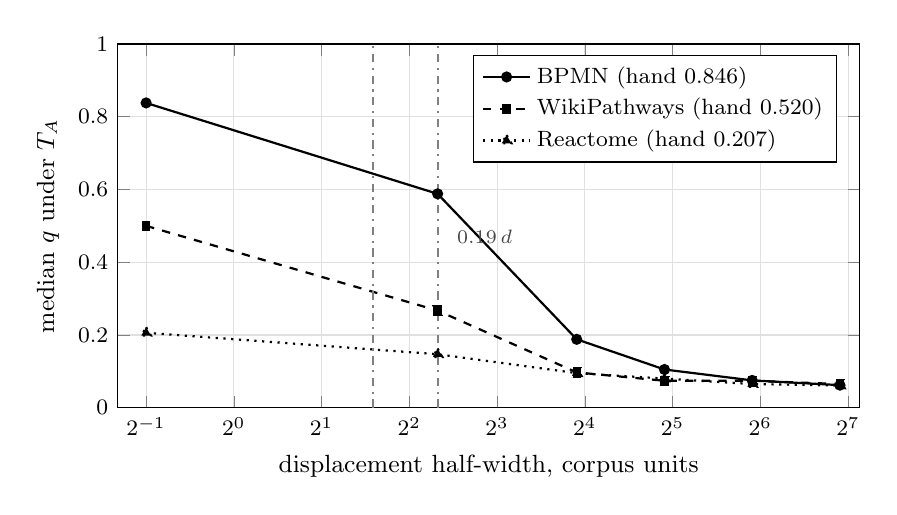
\begin{tikzpicture}
\begin{axis}[width=11cm,height=6.2cm,
  xmode=log,log basis x=2,
  xlabel={displacement half-width, corpus units},
  ylabel={median $q$ under $T_A$},
  ymin=0,ymax=1,xmin=0.4,xmax=140,
  legend pos=north east,legend cell align=left,
  grid=major,grid style={black!12},
  tick label style={font=\footnotesize},label style={font=\small},
  legend style={font=\footnotesize}]
\addplot[thick,mark=*,mark size=1.6pt] coordinates
  {(0.5,0.838)(5,0.588)(15,0.188)(30,0.105)(60,0.075)(120,0.062)};
\addlegendentry{BPMN (hand 0.846)}
\addplot[thick,mark=square*,mark size=1.5pt,dashed] coordinates
  {(0.5,0.500)(5,0.267)(15,0.097)(30,0.074)(60,0.074)(120,0.065)};
\addlegendentry{WikiPathways (hand 0.520)}
\addplot[thick,mark=triangle*,mark size=2pt,dotted] coordinates
  {(0.5,0.206)(5,0.147)(15,0.095)(30,0.080)(60,0.065)(120,0.061)};
\addlegendentry{Reactome (hand 0.207)}
\addplot[gray,thick,dash dot,forget plot] coordinates {(3,0)(3,1)};
\addplot[gray,thick,dash dot,forget plot] coordinates {(5,0)(5,1)};
\node[anchor=west,font=\scriptsize,gray!55!black] at (axis cs:5.4,0.47) {$0.19\,d$};
\end{axis}
\end{tikzpicture}
\caption{The displacement sweep, every box of every hand layout displaced by up to the
half-width, the alignment hold read at $d = 0.02$ and sixteen directions. The declared
half-pitch test sits at the left edge, 0.5 units, where nothing has changed: the corner of
$T_A$ releases a box only past $0.19\,d$, 3 units in the biological corpora and 5 in
BPMN. Past the bound the hold falls, BPMN 0.84 to 0.59 by a half-width of 5, and by 120
units every corpus is at the grid-snapped level of 0.06 to 0.09.}
\label{fig:sweep}
\end{figure}


\section*{S8\quad The plan and its outcomes}

The plan of 22 August 2026 (\texttt{PLAN-STATIONARITY.md}, signed that day) fixed its
hypotheses after a 60-diagram pilot the same morning, so they carried no risk once the
pilot had run, and the paper does not claim a registration. Its hypotheses and what the run found:

\begin{center}\small
\begin{tabular}{@{}p{1cm}>{\raggedright\arraybackslash}p{7.6cm}>{\raggedright\arraybackslash}p{5.6cm}@{}}
\toprule
& hypothesis & outcome \\
\midrule
H1 & under $C{+}O$ the hand layout is held, median $q$ above 0.9 in every corpus & held: 1.00 \\
H2 & under $T_L$ alone it is not, median below 0.2 & held: 0.00; also true of every non-optimised layout \\
H3 & no positive weight on $T_L$ repairs $C{+}O{+}L$ & held: the step of Section~4 \\
H4 & alignment holds more hand-placed boxes than orthogonality or node--edge separation, and more than the tool control & refuted on the held fraction: node--edge holds 0.88 to 1.00 against alignment's 0.21 to 0.85; held on the value against \texttt{neato} and on the hold against \texttt{neato}; below \texttt{dot} \\
H5 & under stress alone the hand layout is held less than \texttt{neato}'s & held: 0.00 against 1.00 \\
\bottomrule
\end{tabular}
\end{center}

Departures from the plan, all recorded after the analyses they concern: the plan's
primary alignment definition is gridiness, and the paper reports the gridiness value with
the A1 hold beside it; the flow term, declared
as an alternative, is measured as a criterion; the reading direction is fitted like $L$;
ELK, logged as unavailable, was obtained and run; the paired control is \texttt{dot}
rather than \texttt{neato} and the test two-sided rather than one-sided (S5); the multiplicity
family is the terms within one corpus against one control; the BPMN sample is the random
300 of Section~S6; the radius in box widths, the A2 alignment definition
and containment as a hard constraint, all declared, were not run.


{\footnotesize
\begin{thebibliography}{9}
\bibitem{bergstra12} J.~Bergstra, Y.~Bengio. Random Search for Hyper-Parameter
 Optimization. \emph{Journal of Machine Learning Research} 13:281--305, 2012.
\bibitem{jw95} A.~Juels, M.~Wattenberg. Stochastic Hillclimbing as a Baseline Method for
 Evaluating Genetic Algorithms. \emph{Advances in Neural Information Processing Systems 8}
 (NIPS 1995), MIT Press, 430--436, 1996.
\end{thebibliography}}

\end{document}
